\section{The Machine Learning Models}
\subsection{Model selection}
In this analysis I have chosen to compare 4 different \ac{ML}-models, dens-\acf{NN}, \acf{PNN},
\ac{LWTA} and XGBoost. The first three methods are all types of \ac{NN}. I have deliberately 
chosen to focus on \ac{NN} given that there is far more freedom in the design of the architecture
of a \ac{NN}, than compared to a XGboost. Additionally, this was motivated by the selfish reason
being that I found the networks more interesting to study and dissect. Therefore, most of the 
analysis, comparisons and discussion is focused on the networks, while XGBoost is included 
as a loose benchmark. 
\\
The choice of the three network architectures is motivated in wanting to compare a simple 
deep network, a network ensemble and a \ac{PNN}. I would assume that the optimal architecture
would be a network which combines elements from each, but for the purpose of discussion
and research I have chosen to keep them somewhat separate. 
\subsection{Creating custom layers}\label{subsec:CustomLayer}
The field of \ac{ML} is one of the most dynamic and fastest growing fields of research
today. This means, that regardless of the brave attempt made by voluntary contributors and
the people at Google\footnote{The developers of TensorFlow}, there will always be 
new and exciting \ac{ML} tools, not yet implemented in their library. This was also 
the case in this thesis. Specifically, in the case of non-dense layers I was forced
to dive into the world of \ac{ML} development and create my own implementation. 
\subsubsection*{Max-out}
TensorFlow have already implemented a very similar layer called MaxPooling1D. This does 
exactly what max-out (see subsection \ref{subsubsec:maxout}) does, but with minor differences. 
Additionally, I wanted the freedom to experiment with the implementation of the layer. The 
implementation of both max-out and channel-out (see subsection \ref{subsubsec:channelout}) 
was done by creating a custom activation function which is called inside a dense-layer. 
\\
In the code listing, \ref{lst:max_out} I have included the code implementation of the
activation function used to create the max-out layer. The listing shows how the function
takes the input from the previous layer, defines the new shape of what will become the 
output, groups the nodes in the size defined by number of units, then returns an output 
which includes only the largest activated node from each unit. By using this function 
in a dense-layer, said layer will act as a max-out layer. 

\begin{algorithm}
    \caption{The pseudo code for implementing the Maxout layer in TensorFlow}\label{alg:maxout}
    \begin{algorithmic}[1]
    \State def \textbf{MaxOut}(Input): 
    \State \ \ \ \ $\%$ Pass input through weight kernel and adding bias terms
    \State \ \ \ \ $Input \gets Input \times Weights$
    \State \ \ \ \ $Input \gets Input + Bias$
    \\
    \State \ \ \ \ $\%$ Reshape input into units
    \State \ \ \ \ $Input \gets \textbf{Reshape}(Input,(Nr\ Units,\ Size \ of \ Units))$
    \\
    \State \ \ \ \ $\%$ Reduce input to the largest activation in each unit
    \State \ \ \ \ $Output \gets \textbf{Max}(Input)$
    \\
    \State \ \ \ \ $\%$ Reshape to size equal the number of units.
    \State \ \ \ \ $Output \gets \textbf{Reshape}(Input,(Nr \ Units))$
    \State \ \ \ \ $\textbf{return}\ Input$
    \end{algorithmic}
\end{algorithm}

\subsubsection*{Channel-out}
For the activation function defined to create the channel-out layer, I again grouped
the nodes similarly as I did for max-out. Instead of returning the largest value from each 
unit, I used TensorFlow's function, $tf.greater\_equal$ to create a tensor with booleans. The 
booleans are chosen by comparing each unit to the largest value in that unit. By multiplying 
this tensor to the original input, I am left with the desired result of a tensor containing 
the largest activated nodes along with the rest whom are now set to zero. 
\begin{algorithm}
    \caption{The pseudo code for implementing the channel-out layer in TensorFlow}\label{alg:channel-out}
    \begin{algorithmic}[1]
    \State def \textbf{Channel-out}(Input): 
    \State \ \ \ \ $\%$ Pass input through weight kernel and adding bias terms.
    \State \ \ \ \ $Input \gets Input \times Weights$
    \State \ \ \ \ $Input \gets Input + Bias$
    \\
    \State \ \ \ \ $\%$ Reshape input into units
    \State \ \ \ \ $Input \gets \textbf{Reshape}(Input,(Nr\ Units,\ Size \ of \ Units))$
    \\
    \State \ \ \ \ $\%$ Reduce input to the largest activation in each unit.
    \State \ \ \ \ $Output \gets \textbf{Max}(Input)$
    \\
    \State \ \ \ \ $\%$ Set original activation where activation is largest and 0 where it's not.
    \State \ \ \ \ $Output \gets \textbf{Where}(Input == Output, Input,0)$
    \\
    \State \ \ \ \ $\%$ Reshape to original size.
    \State \ \ \ \ $Output \gets \textbf{Reshape}(Output,(Input's \ Original \ Shape))$
    \State \ \ \ \ $\textbf{return}\ Output$
    \end{algorithmic}
\end{algorithm}
\subsubsection*{\ac{SCO}}
In section \ref{subsubsec:stochchannelout} I described how \ac{SCO} is an extension of channel-out. The only difference
between the two, is that \ac{SCO} utilizes dynamic units instead of static. Therefore, when creating the \ac{SCO} layer,
the only change needed was grouping the nodes differently for each prediction. This was implemented by 
\begin{algorithm}
    \caption{The pseudo code for implementing the SCO layer in TensorFlow}\label{alg:SCO}
    \begin{algorithmic}[1]
    \State def \textbf{SCO}(Input): 
    \State \ \ \ \ $\%$ Pass input through weight kernel and adding bias terms.
    \State \ \ \ \ $Input \gets Input \times Weights$
    \State \ \ \ \ $Input \gets Input + Bias$
    \\
    \State \ \ \ \ $\%$ Shuffle all the values
    \State \ \ \ \ $InputShuflle \gets \textbf{Shuffle}(Input)$
    \\
    \State \ \ \ \ $\%$ Reshape input into units
    \State \ \ \ \ $InputShuflle \gets \textbf{Reshape}(InputShuflle,(Nr\ Units,\ Size \ of \ Units))$
    \\
    \State \ \ \ \ $\%$ Reduce input to the largest activation in each unit.
    \State \ \ \ \ $OutputShuffle \gets \textbf{Max}(InputShuflle)$
    \\
    \State \ \ \ \ $\%$ Set 1 where activation is largest and 0 where not.
    \State \ \ \ \ $OutputShuffle \gets \textbf{Where}(InputShuflle == OutputShuffle, 1,0)$
    \\
    \State \ \ \ \ $\%$ Un-shuffle all the values
    \State \ \ \ \ $Output \gets \textbf{UnShuffle}(Input)$
    \\
    \State \ \ \ \ $\%$ Reshape to original size.
    \State \ \ \ \ $Output \gets \textbf{Reshape}(Output,(Input's \ Original \ Shape))$
    \\
    \State \ \ \ \ $\%$ Multiply input with output to set all input that are not the largest, to zero.
    \State \ \ \ \ $Input \gets Input \times Output$
    \\
    \State \ \ \ \ $\textbf{return}\ Input$
    \end{algorithmic}
\end{algorithm}
\subsection{Model Architecture}
When choosing a network architecture, there are several ways to proceed. One way is to apply a grid search.
A grid search is simply defining a grid of parameters to test, then running through all combinations and 
choosing the highest performer. With a sufficient amount of tests, a grid search should converge towards 
an optimal architecture. Grid search is very common and there exists a large range of very complex varieties \cite{GS}.
For my analysis I chose not to perform a grid search, for several reasons. The first being interpretability.
Understanding a \ac{NN} is already hard, allowing for complex and unique architectures would only add another layer
of mysticism. The second is the size of the data set. The larger the data set, the larger the amount of data 
would be needed to adequately perform tests for each combination of parameters. Not only is this time-consuming,
but trying to mediate this issue could lead to poor performance. The third and most important reason is that 
I wanted to experiment with the architectures. By manually tuning the parameters, I was able to achieve a far 
better understanding of the final architecture. 
\begin{figure}
    \makebox[0.9\linewidth][c]{%
    \centering
    \begin{subfigure}{1.1\textwidth}
        \centering
        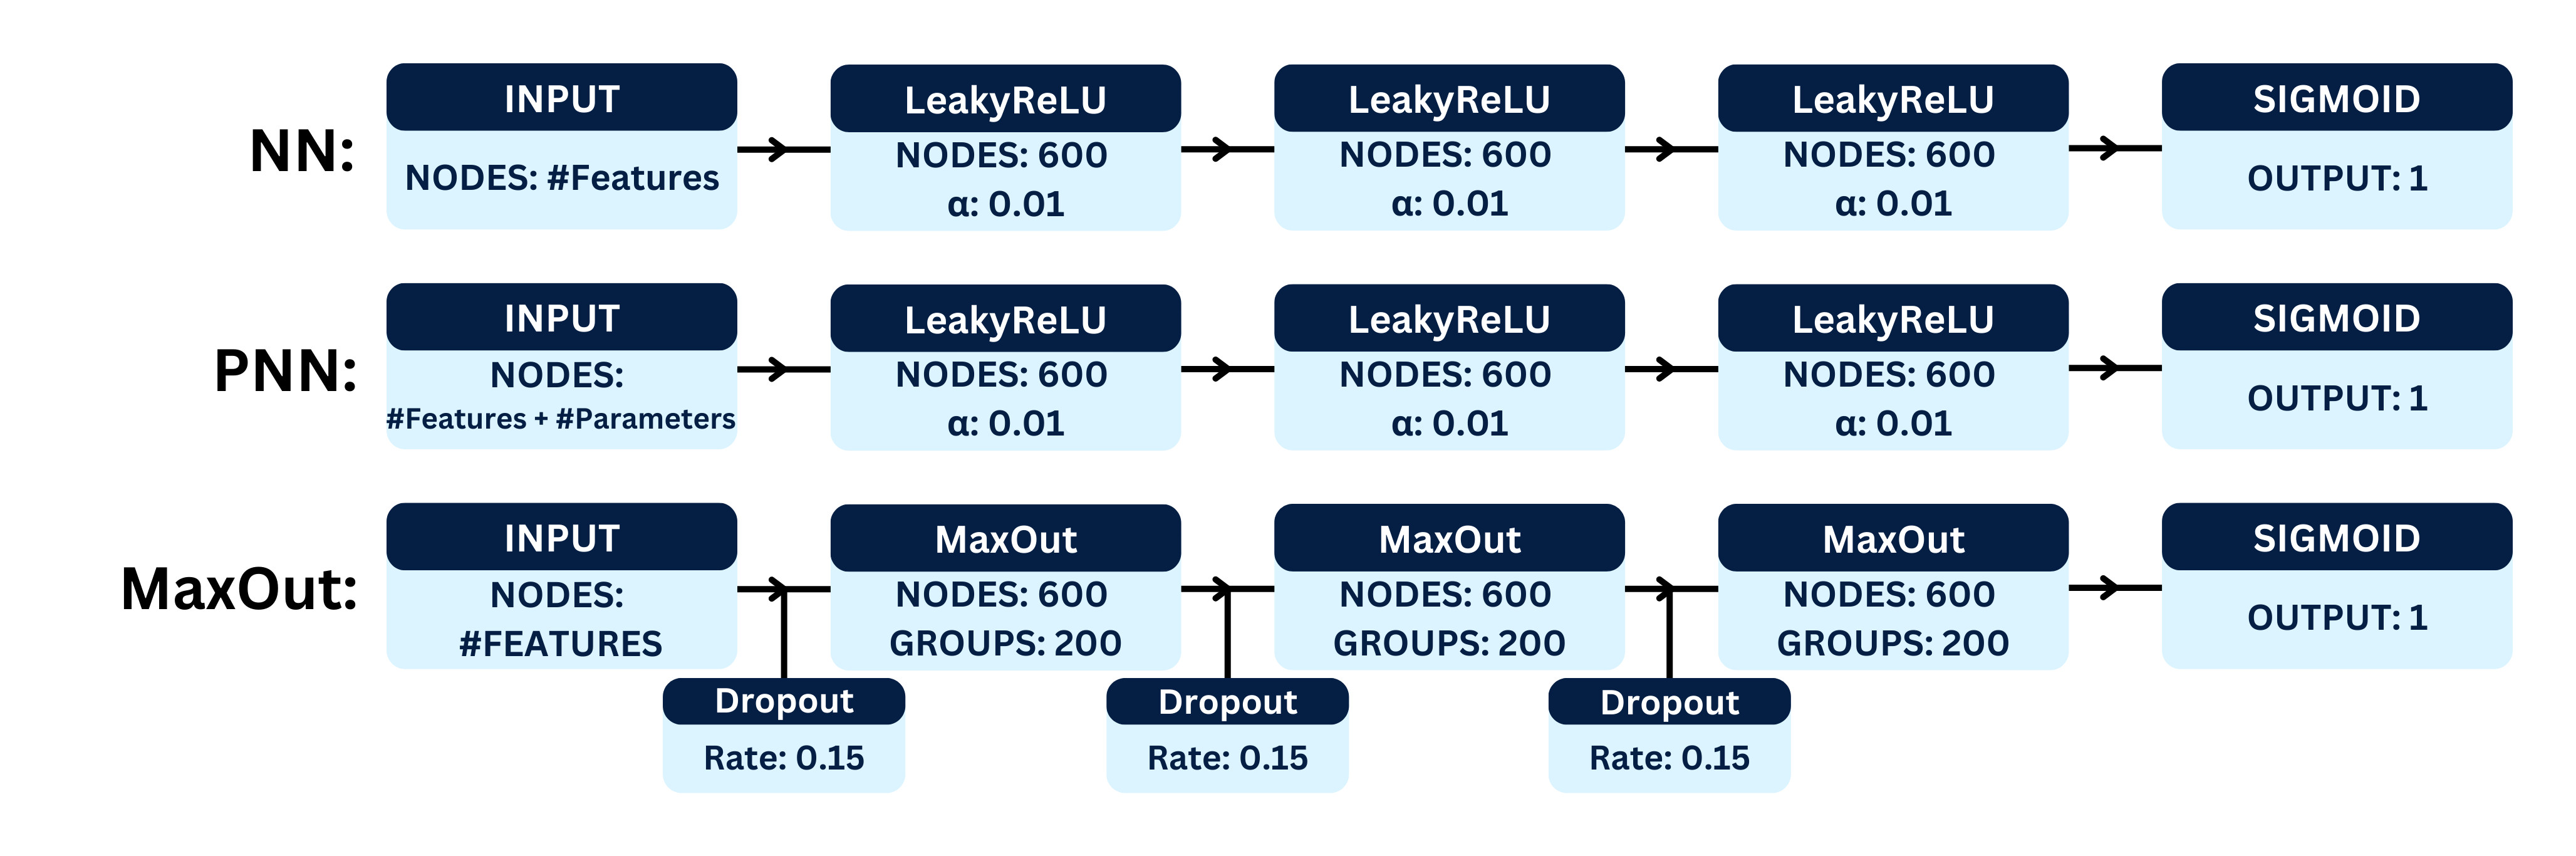
\includegraphics[width=\textwidth]{Figures/Illustrations/architecture.png}
    \end{subfigure}
    }
    \caption{A visual summary of the workflow and framework use for the 
    computational analysis. }
    \label{fig:arch}
\end{figure}
\subsection*{Dense Neural Network and PNN}\label{subsec:PNNArch}
The purpose of the simple dense \ac{NN}, is to compare the more complex networks to what is usually considered a traditional \ac{NN}.
All layers are dense layers, meaning that all nodes in the previous layer are connected to the current layer, and likewise
the current layer is connected to the next. The general structure of the network is summarized in figure \ref{fig:arch}, with 
the network label \ac{NN}\footnote{Note that the dense network will henceforth be referred to as \ac{NN}}. The figure shows a \ac{DNN} with 
three hidden layers, all with 600 nodes each. All hidden layers utiliz the $LeakyReLU$ activation (see section \ref{subsec:activation})
with an $\alpha$ = 0.01. The architecture is designed to perform deep-training, and will train on a training set where all mass combinations 
are included\footnote{Contrary to training one network for each mass combination.}. 
\\
The \ac{PNN} architecture is like the name suggests, included to represent the model proposed by the article by Baldi et al. \cite{PNN}.
The architecture is illustrated in figure \ref{fig:arch}, with the label PNN. The figure shows a practically identical 
structure to the dense-\ac{NN}, with the only difference being in the input-layer. As was discussed in section \ref{subsec:PNN},
the \ac{PNN} includes the new physics signal free parameters\footnote{In our case, the masses of the \ac{BSM}-particles.} alongside the features
in the input layer.
\subsection*{MaxOut, Channel-Out and \ac{SCO}}
The ensemble methods are slightly than both the dense \ac{NN} and \ac{PNN} in terms of architecture. To limit the complexity for comparison reasons
I choose to build an identical architecture for maxout, channel-Out and \ac{SCO}, with the only difference being which of the three layers is used.  
In figure \ref{fig:arch} I have illustrated the MaxOut architecture, with the label MaxOut. The figure shows a network with 6 hidden layers, 
3 MaxOut and 3 dropout. The network alternates between drop out and MaxOut, starting with dropout and finishing with MaxOut. The MaxOut layers 
have 600 nodes each which reduce down to the 200 nodes with the largest activation in their respective groups. Each dropout layer has a dropout 
rate of 0.15. Channel-out and \ac{SCO} have the same architecture to maxout, but replacing maxout with the two respectively. 

\subsection*{XGBoost}\label{subsec:XGBoost}
The main motivation to apply XGBoost is simply to benchmark my analysis, and therefore not a lot of effort has been put into the design of the 
architecture. Therefore, the default parameters\footnote{See \href{https://xgboost.readthedocs.io/en/stable/parameter.html}
{https://xgboost.readthedocs.io/en/stable/parameter.html}
for a complete overview of default parameters.} of XGBoost has been used. The main parameters of the model are summarized as the following:
\begin{itemize}
    \item $\eta$ (learning-rate) = 0.3
    \item Max depth = 6
    \item Maximum number of trees = 100
\end{itemize}

